% Options for packages loaded elsewhere
\PassOptionsToPackage{unicode}{hyperref}
\PassOptionsToPackage{hyphens}{url}
\PassOptionsToPackage{dvipsnames,svgnames,x11names}{xcolor}
\documentclass[
  10pt,
  fontset=fandol]{ctexart}
\usepackage{xcolor}
\usepackage[margin=16mm]{geometry}
\usepackage{amsmath,amssymb}
\setcounter{secnumdepth}{-\maxdimen} % remove section numbering
\usepackage{iftex}
\ifPDFTeX
  \usepackage[T1]{fontenc}
  \usepackage[utf8]{inputenc}
  \usepackage{textcomp} % provide euro and other symbols
\else % if luatex or xetex
  \usepackage{unicode-math} % this also loads fontspec
  \defaultfontfeatures{Scale=MatchLowercase}
  \defaultfontfeatures[\rmfamily]{Ligatures=TeX,Scale=1}
\fi
\usepackage{lmodern}
\ifPDFTeX\else
  % xetex/luatex font selection
\fi
% Use upquote if available, for straight quotes in verbatim environments
\IfFileExists{upquote.sty}{\usepackage{upquote}}{}
\IfFileExists{microtype.sty}{% use microtype if available
  \usepackage[]{microtype}
  \UseMicrotypeSet[protrusion]{basicmath} % disable protrusion for tt fonts
}{}
\makeatletter
\@ifundefined{KOMAClassName}{% if non-KOMA class
  \IfFileExists{parskip.sty}{%
    \usepackage{parskip}
  }{% else
    \setlength{\parindent}{0pt}
    \setlength{\parskip}{6pt plus 2pt minus 1pt}}
}{% if KOMA class
  \KOMAoptions{parskip=half}}
\makeatother
\usepackage{graphicx}
\makeatletter
\newsavebox\pandoc@box
\newcommand*\pandocbounded[1]{% scales image to fit in text height/width
  \sbox\pandoc@box{#1}%
  \Gscale@div\@tempa{\textheight}{\dimexpr\ht\pandoc@box+\dp\pandoc@box\relax}%
  \Gscale@div\@tempb{\linewidth}{\wd\pandoc@box}%
  \ifdim\@tempb\p@<\@tempa\p@\let\@tempa\@tempb\fi% select the smaller of both
  \ifdim\@tempa\p@<\p@\scalebox{\@tempa}{\usebox\pandoc@box}%
  \else\usebox{\pandoc@box}%
  \fi%
}
% Set default figure placement to htbp
\def\fps@figure{htbp}
\makeatother
\setlength{\emergencystretch}{3em} % prevent overfull lines
\providecommand{\tightlist}{%
  \setlength{\itemsep}{0pt}\setlength{\parskip}{0pt}}
\usepackage{amsmath,amssymb,mathtools,needspace}
\xeCJKDeclareCharClass{CJK}{"2032,"0400->"04FF,"2160->"216B,"2460->"2473,"25A0,"25C7,"25CB,"25CF}
\IfFontExistsTF{Arial Unicode MS}{\xeCJKsetup{AutoFallBack=true}\setCJKfallbackfamilyfont{\CJKrmdefault}{Arial Unicode MS}}{}
\setcounter{secnumdepth}{0}
\setlength{\emergencystretch}{2em}
\allowdisplaybreaks
\usepackage{bookmark}
\IfFileExists{xurl.sty}{\usepackage{xurl}}{} % add URL line breaks if available
\urlstyle{same}
\hypersetup{
  pdftitle={快速变换 FWT},
  colorlinks=true,
  linkcolor={Maroon},
  filecolor={Maroon},
  citecolor={Blue},
  urlcolor={Blue},
  pdfcreator={LaTeX via pandoc}}

\title{快速变换 FWT}
\author{}
\date{}

\begin{document}
\maketitle

\subsection{10.4　快速变换 FWT}\label{ux5febux901fux53d8ux6362-fwt}

不同排序方式的 Walsh 变换，其快速算法的设计方法彼此类同。本节将着重考察 Hadamard 序的 Walsh 变换 \(N\)-WT

\[
X(i)=\sum_{j=0}^{N-1}x(j)H_N(i,j),\quad i=0,1,\cdots,N-1,
\tag{10.4.1}
\]

式中，\(H_N\) 为 \(N\) 阶 Hadamard 阵，\(\{x(j)\}_0^{N-1}\) 为输入数据，输出数据 \(\{X(i)\}_0^{N-1}\) 待求。这里仍然假定 \(N=2^n\)，\(n\) 为正整数。

由于 Hadamard 阵是对称正交阵，Walsh 变换（10.4.1）同它的逆变换

\[
x(j)=\frac1N\sum_{i=0}^{N-1}X(i)H_N(i,j),\quad j=0,1,\cdots,N-1
\]

仅仅相差一个常数因子，因此两者可以统一加以考察。

本节将基于定理 10.1 设计 Walsh 变换（10.4.1）的快速算法 FWT。

\begin{quote}
校注（agent 补充，CH10-E002）：原文``对称正交阵''照录。依本章未归一化的 \(\pm1\) 元素定义，\(H_N^\mathsf{T}H_N=NI\)，\(N>1\) 时并非通常定义下满足 \(Q^\mathsf{T}Q=I\) 的正交矩阵；准确地说其行列两两正交，\(H_N/\sqrt N\) 才是正交矩阵。原页逆变换中的 \(1/N\) 因子与该定义一致。本项是原书术语疑误，不是 OCR 错误。
\end{quote}

\subsubsection{10.4.1　FWT 的设计思想}\label{fwt-ux7684ux8bbeux8ba1ux601dux60f3}

在具体设计快速算法 FWT 之前，首先考察两种简单情形。由于 1 阶和 2 阶 Hadamard 阵为

\[
H_1=[\,+\,],
\]

\[
H_2=\begin{pmatrix}+&+\\+&-\end{pmatrix},
\]

因而 1-WT 具有极其简单的形式

\[
X(0)=x(0).
\]

这里输入数据即为所求结果，因而不需要做任何计算。此外，2-WT 为

\[
\begin{cases}
X(0)=x(0)+x(1),\\
X(1)=x(0)-x(1).
\end{cases}
\]

这项计算也很平凡，不存在算法设计问题。

可见，1-WT 与 2-WT 都是极为简单的。

\textbf{快速算法 FWT 的设计思想是，基于规模减半的二分手续，通过 2-WT 的反复计算，将所给 \(N\)-WT 逐步加工成 1-WT，从而得出所求的结果。}

快速算法 FWT 是优秀算法的一朵奇葩，它鲜明地展现了``简单的重复生成复杂''这一算法设计的基本理念。此外，它可以充当一个样板，示范运用二分演化机制设

\href{../../source-images/pdf-271.jpeg}{原页}

计快速变换的全过程。

\subsubsection{10.4.2　FWT 的演化机制}\label{fwt-ux7684ux6f14ux5316ux673aux5236}

前已反复指出，二分技术是快速算法设计的基本技术。二分技术的基本点是运用某种二分手续，将所给计算问题化归为规模减半的同类问题。

对于 \(N\) 点 Walsh 变换 \(N\)-WT（10.4.1），即

\[
X(i)=\sum_{j=0}^{N-1}x(j)H_N(i,j),\quad i=0,1,\cdots,N-1.
\]

将其右端的和式对半拆开，有

\[
\begin{aligned}
X(i)&=\sum_{j=0}^{N/2-1}x(j)H_N(i,j)+\sum_{j=N/2}^{N-1}x(j)H_N(i,j)\\
&=\sum_{j=0}^{N/2-1}[x(j)H_N(i,j)+x(N/2+j)H_N(i,N/2+j)],\quad i=0,1,\cdots,N-1.
\end{aligned}
\]

然后再将这组算式对半分为两组算式，有

\[
\begin{cases}
\displaystyle X(i)=\sum_{j=0}^{N/2-1}[x(j)H_N(i,j)+x(N/2+j)H_N(i,N/2+j)],\\[6pt]
\displaystyle X(N/2+i)=\sum_{j=0}^{N/2-1}[x(j)H_N(N/2+i,j)+x(N/2+j)H_N(N/2+i,N/2+j)],
\end{cases}
\]

\[
i=0,1,\cdots,N/2-1.
\]

利用定理 1 的递推关系将上述算式化简，得

\[
\begin{cases}
\displaystyle X(i)=\sum_{j=0}^{N/2-1}[x(j)+x(N/2+j)]H_{N/2}(i,j),\\[6pt]
\displaystyle X(N/2+i)=\sum_{j=0}^{N/2-1}[x(j)-x(N/2+j)]H_{N/2}(N/2+i,j),
\end{cases}\quad i=0,1,\cdots,N/2-1.
\]

这样，所给 \(N\)-WT（10.4.1）被加工成下列两个 \(N/2\)-WT：

\[
\begin{cases}
\displaystyle X(i)=\sum_{j=0}^{N/2-1}x_1(j)H_{N/2}(i,j),\\[6pt]
\displaystyle X(N/2+i)=\sum_{j=0}^{N/2-1}x_1(N/2+j)H_{N/2}(N/2+i,j),
\end{cases}\quad i=0,1,\cdots,N/2-1.
\]

为此所要施行的二分手续是

\[
\begin{cases}
x_1(j)=x(j)+x(N/2+j),\\
x_1(N/2+j)=x(j)-x(N/2+j),
\end{cases}\quad j=0,1,\cdots,N/2-1
\tag{10.4.2}
\]

上述二分手续将所给 \(N\)-WT 加工成 2 个 \(N/2\)-WT。每个 \(N/2\)-WT 通过二分手续可进一步加工成 2 个 \(N/4\)-WT。如此反复二分，使问题的规模逐次减半，最终可将

\begin{quote}
校注（agent 补充，CH10-E001）：本页化简式及其后两个 \(N/2\)-WT 的第二式，原图均写作 \(H_{N/2}(N/2+i,j)\)，上文已照录。按前页定理 10.1 和本章对 \(N/2\) 阶矩阵的索引范围，这里的行指标 \(N/2+i\) 超出 \(0,\ldots,N/2-1\)；由 \(H_N(N/2+i,j)=H_{N/2}(i,j)\)，两处应为 \(H_{N/2}(i,j)\)。这是原书下标疑误，不是 OCR 错误。\href{../assets/ch10/erratum-p271-indices.png}{原式放大裁片}。此外，本页``定理 1''照录，所用递推关系对应前页``定理 10.1''。
\end{quote}

\href{../../source-images/pdf-272.jpeg}{原页}

\(N\)-WT 加工成 \(N\) 个 1-WT，从而得出所求的结果。这种演化过程

\[
\underset{\text{（计算模型）}}{N\text{-WT}}\Rightarrow2\text{ 个 }N/2\text{-WT}\Rightarrow4\text{ 个 }N/4\text{-WT}\Rightarrow\cdots\Rightarrow\underset{\text{（计算结果）}}{N\text{ 个 }1\text{-WT}}
\]

称作\textbf{快速 Walsh 变换}。这里箭头``\(\Rightarrow\)''表示二分手续（10.4.2）。

进一步剖析二分手续（10.4.2）的内涵，计算模型 \(N\)-WT 所要加工的数据 \(\{x(j)\}\) 是个 \(N\) 维向量，将它对半二分，得 \(N/2\) 个\textbf{平移对} \((x(j),x(N/2+j))\)。可见二分手续（10.4.2）的含义是，将平移对的两个数据相加减，因而 FWT 从属于图 10.5 的二分演化模式。

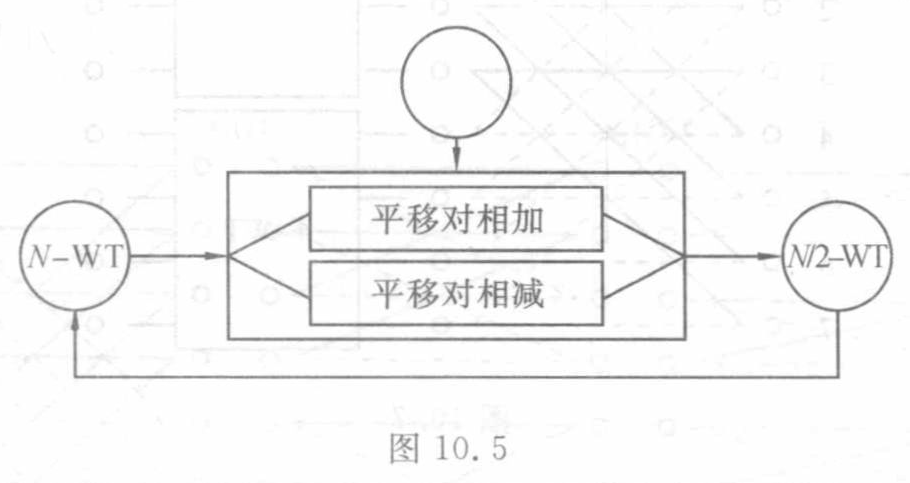
\includegraphics[width=0.85\linewidth,height=\textheight,keepaspectratio,alt={图 10.5（原图裁切）：FWT 的二分演化模式}]{../assets/ch10/fig-10-5.png}

图 10.5

\begin{quote}
图中文字与图意（转录）：左端 \(N\)-WT 进入``平移对相加''和``平移对相减''两路，合成右端 \(N/2\)-WT，底部有返回左端的反馈线；顶部有一个向下接入的空圆，原图未印文字标签。
\end{quote}

最后统计 FWT 的运算量。由于 FWT 的每一步使问题的的规模减半，欲将所给 \(N\)-WT，\(N=2^n\) 加工成 \(N\) 个 1-WT，二分演化需做 \(n=\log_2N\) 步，又形如式（10.4.2）的二分手续的每一步要做 \(N\) 次加减操作，因而 FWT 的总运算量为 \(N\log_2N\) 次加减操作。另一方面，如果直接计算 \(N\)-WT（10.4.1）要做 \(N^2\) 次加减操作，故 FWT 是快速算法，其加速比

\[
\frac{N^2}{N\log_2N}\to\infty\quad\text{（当 }N\to\infty\text{ 时）}.
\]

\subsubsection{10.4.3　FWT 的计算流程}\label{fwt-ux7684ux8ba1ux7b97ux6d41ux7a0b}

二分手续（10.4.2）采取两两加工的处理方式，即将一对数据 \((x(j),x(N/2+j))\) 加工成一对新的数据 \((x_1(j),x_1(N/2+j))\)，其计算格式如图 10.6 所示。这里分别用实线与虚线区分数据的相加与相减两种运算。

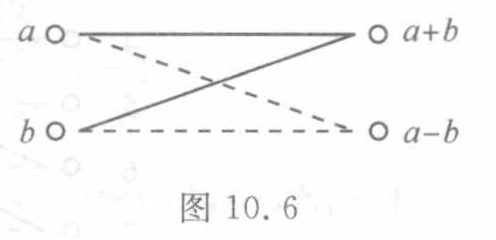
\includegraphics[width=0.85\linewidth,height=\textheight,keepaspectratio,alt={图 10.6（原图裁切）：两两加工的计算格式}]{../assets/ch10/fig-10-6.png}

图 10.6

\begin{quote}
图中文字与图意（转录）：左端输入从上到下为 \(a\)、\(b\)，右端输出从上到下为 \(a+b\)、\(a-b\)。输入至上方输出的两条线为实线，输入至下方输出的两条线为虚线，形成交叉的两两计算格式。
\end{quote}

现在运用二分技术针对 8-WT：

\[
X(i)=\sum_{j=0}^{7}x(j)H_8(i,j),\quad i=0,1,\cdots,7.
\tag{10.4.3}
\]

具体显示前述 FWT 的计算流程。

\textbf{步 1}　施行 \(N=8\) 的二分手续（10.4.2），即

\[
x_1(0)=x(0)+x(4),\quad x_1(4)=x(0)-x(4),
\]

\begin{quote}
校注（agent 补充）：原页``使问题的的规模减半''重复``的''，上文照录。
\end{quote}

\href{../../source-images/pdf-273.jpeg}{原页}

\[
\begin{aligned}
x_1(1)&=x(1)+x(5),& x_1(5)&=x(1)-x(5),\\
x_1(2)&=x(2)+x(6),& x_1(6)&=x(2)-x(6),\\
x_1(3)&=x(3)+x(7),& x_1(7)&=x(3)-x(7),
\end{aligned}
\]

将所给 8-WT 加工成 2 个 4-WT。借助于图 10.6 的计算格式，这一演化步骤如图 10.7 所示。

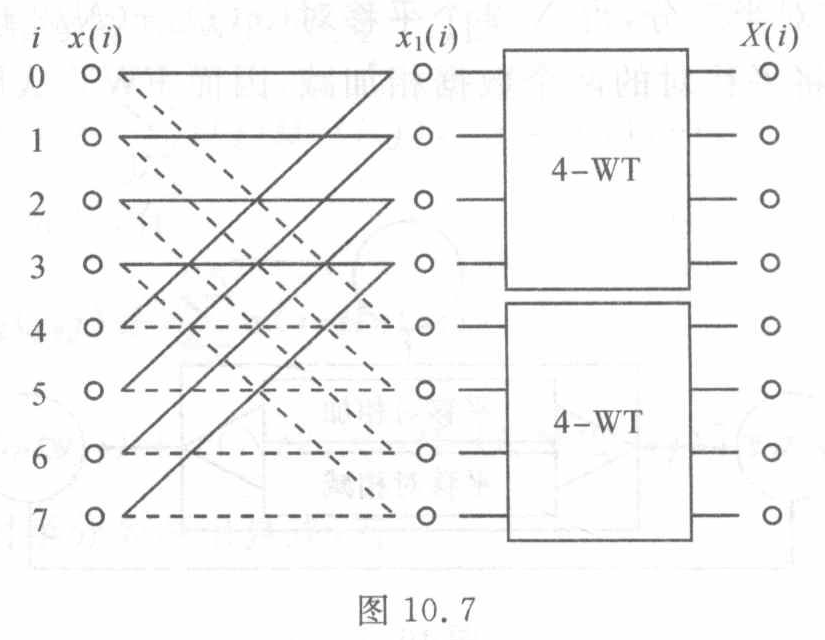
\includegraphics[width=0.85\linewidth,height=\textheight,keepaspectratio,alt={图 10.7（原图裁切）：8-WT 经第一步化成两个 4-WT}]{../assets/ch10/fig-10-7.png}

图 10.7

\begin{quote}
图中文字与图意（转录）：从左到右的列标为 \(i\)、\(x(i)\)、\(x_1(i)\)、\(X(i)\)。\(i\) 的行标为 0、1、2、3、4、5、6、7；两组模块均标为 4-WT。第一个加工阶段将行对 \((0,4)\)、\((1,5)\)、\((2,6)\)、\((3,7)\) 相加减，所得 \(x_1(i)\) 的前四项、后四项分别接入一个 4-WT，右端输出 \(X(i)\)。
\end{quote}

\textbf{步 2}　对 2 个 4-WT 分别施行 \(N=4\) 的二分手续（10.4.2），即

\[
\begin{aligned}
x_2(0)&=x_1(0)+x_1(2),& x_2(2)&=x_1(0)-x_1(2),\\
x_2(1)&=x_1(1)+x_1(3),& x_2(3)&=x_1(1)-x_1(3)
\end{aligned}
\]

与

\[
\begin{aligned}
x_2(4)&=x_1(4)+x_1(6),& x_2(6)&=x_1(4)-x_1(6),\\
x_2(5)&=x_1(5)+x_1(7),& x_2(7)&=x_1(5)-x_1(7),
\end{aligned}
\]

进一步加工出关于数据 \(\{x_2(j)\}\) 的 4 个 2-WT。这一演化步如图 10.8 所示。

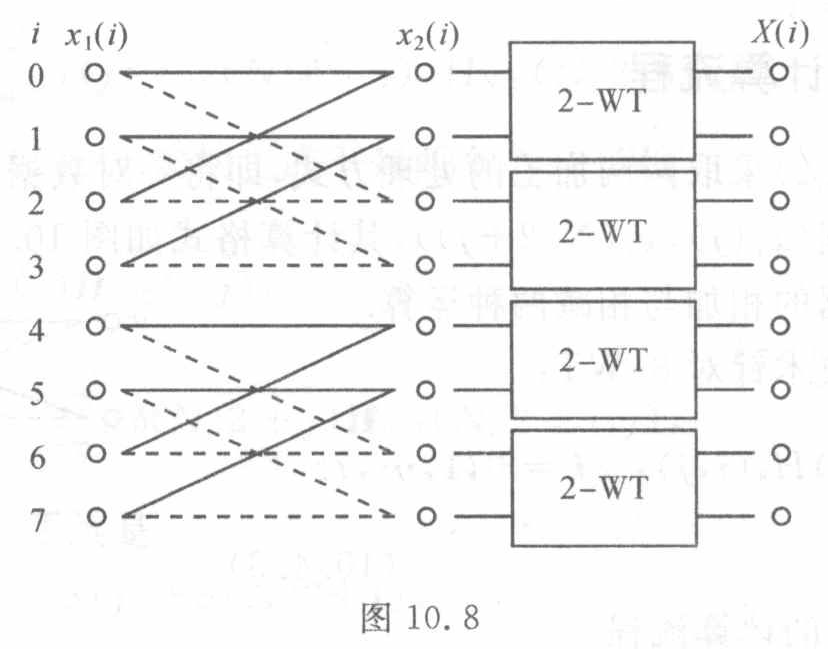
\includegraphics[width=0.85\linewidth,height=\textheight,keepaspectratio,alt={图 10.8（原图裁切）：两个 4-WT 经第二步化成四个 2-WT}]{../assets/ch10/fig-10-8.png}

图 10.8

\begin{quote}
图中文字与图意（转录）：从左到右的列标为 \(i\)、\(x_1(i)\)、\(x_2(i)\)、\(X(i)\)。\(i\) 的行标为 0、1、2、3、4、5、6、7；四组模块均标为 2-WT。该阶段将行对 \((0,2)\)、\((1,3)\)、\((4,6)\)、\((5,7)\) 相加减，所得 \(x_2(i)\) 每两项接入一个 2-WT，右端输出 \(X(i)\)。
\end{quote}

\textbf{步 3}　再对每个 2-WT 分别施行二分手续，即

\href{../../source-images/pdf-274.jpeg}{原页}

\[
\begin{aligned}
x_3(0)&=x_2(0)+x_2(1),& x_3(1)&=x_2(0)-x_2(1),\\
x_3(2)&=x_2(2)+x_2(3),& x_3(3)&=x_2(2)-x_2(3),\\
x_3(4)&=x_2(4)+x_2(5),& x_3(5)&=x_2(4)-x_2(5),\\
x_3(6)&=x_2(6)+x_2(7),& x_3(7)&=x_2(6)-x_2(7).
\end{aligned}
\]

加工得出关于数据 \(\{x_3(i)\}\) 的 8 个 1-WT，即得所求结果：

\[
X(i)=x_3(i),\quad i=0,1,\cdots,7.
\]

上述算法 FWT，其计算模型与输入数据同步进行加工，在将计算模型从 8-WT 加工成 1-WT 的同时，输入数据被加工成输出结果 \(\{X(i)\}\)。综合上述各步即得 FWT 的数据加工流程图 10.9。

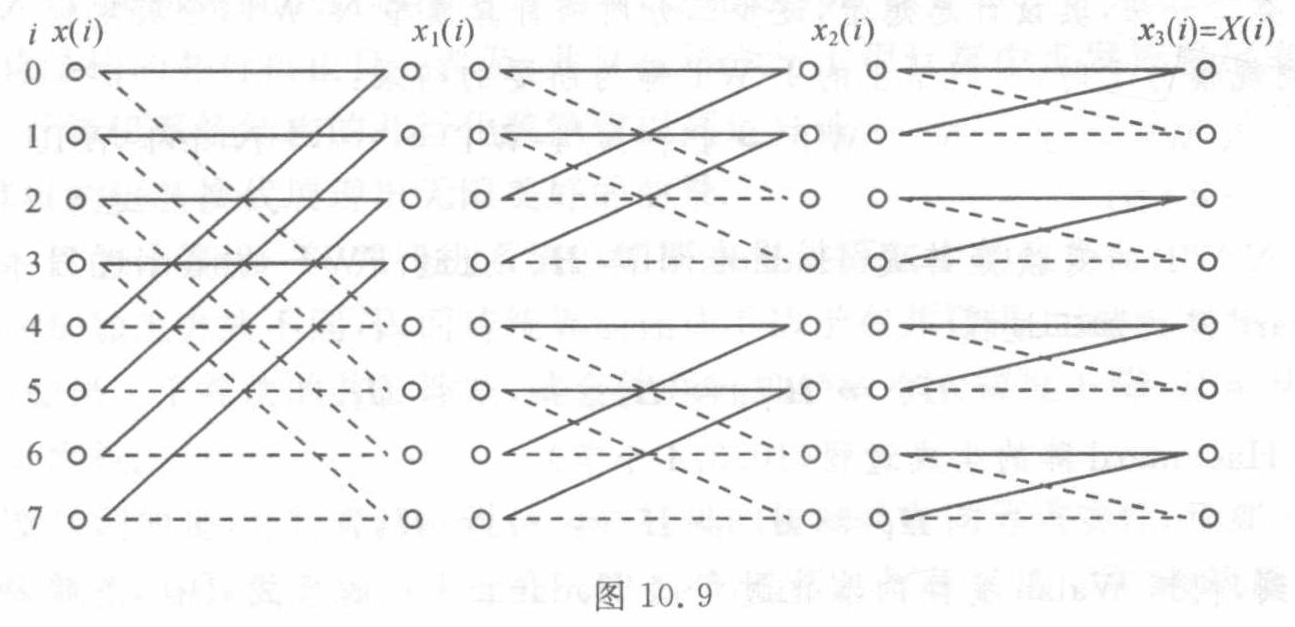
\includegraphics[width=0.85\linewidth,height=\textheight,keepaspectratio,alt={图 10.9（原图裁切）：8-WT 的完整数据加工流程}]{../assets/ch10/fig-10-9.png}

图 10.9

\begin{quote}
图中文字与图意（转录）：列标依次为 \(i\)、\(x(i)\)、\(x_1(i)\)、\(x_2(i)\)、\(x_3(i)=X(i)\)，行标为 0、1、2、3、4、5、6、7。第一阶段配对 \((0,4)\)、\((1,5)\)、\((2,6)\)、\((3,7)\)；第二阶段配对 \((0,2)\)、\((1,3)\)、\((4,6)\)、\((5,7)\)；第三阶段配对 \((0,1)\)、\((2,3)\)、\((4,5)\)、\((6,7)\)。每对按图 10.6 的实线相加、虚线相减计算，三步后由 \(x_3(i)\) 得到 \(X(i)\)。
\end{quote}

\subsubsection{10.4.4　FWT 的算法实现}\label{fwt-ux7684ux7b97ux6cd5ux5b9eux73b0}

回头考察一般形式的 Walsh 变换 \(N\)-WT（10.4.1）。仍设 \(N=2^n\)，\(n\) 为正整数。前已指出，其快速算法设计分 \(n=\log_2N\) 步，每一步将计算问题的规模减半。记 \(N_k=N/2^k\)。快速 Walsh 变换 FWT 的第 \(k\) 步将所给 \(N\)-WT 化归为 \(2^k\) 个 \(N_k\)-WT，其输入数据 \(x_k(i)\) 被分割成 \(2^k\) 段，每段含有 \(N_k\) 个数据，具体地说，其 \(l\)（\(l=1,2,\cdots,2^k\)）段数据为

\[
x_k((l-1)N_k+j),\quad j=0,1,\cdots,N_k-1.
\]

这样，二分过程的第 \(k\) 步是先将 \(k-1\) 步生成的数据段

\[
x_{k-1}((l-1)N_{k-1}+j),\quad j=0,1,\cdots,N_{k-1}-1
\]

再对半切成两部分，其前半部分与后半部分分别是

\[
x_{k-1}((l-1)N_{k-1}+j);\quad x_{k-1}((l-1)N_{k-1}+N_k+j),\quad j=0,1,\cdots,N_k-1.
\]

然后将这两组数据按式（10.4.2）进行加工，结果有

\[
\begin{gathered}
\begin{cases}
x_k((l-1)N_{k-1}+j)=x_{k-1}((l-1)N_{k-1}+j)+x_{k-1}((l-1)N_{k-1}+N_k+j),\\
x_k((l-1)N_{k-1}+N_k+j)=x_{k-1}((l-1)N_{k-1}+j)-x_{k-1}((l-1)N_{k-1}+N_k+j),
\end{cases}\\
j=0,1,\cdots,N_k-1;\quad l=1,2,\cdots,2^k.
\end{gathered}
\tag{10.4.4}
\]

\begin{quote}
校注（agent 补充，CH10-E004）：式（10.4.4）原印 \(l=1,2,\cdots,2^k\)，上文照录。此式用 \((l-1)N_{k-1}\) 定位第 \(k-1\) 步的数据段，该步只有 \(2^{k-1}\) 段，因此上限应为 \(2^{k-1}\)。例如 \(N=8,k=1\) 时，按原印取 \(l=2\) 会访问从索引 8 开始的数据，越过 \(0,\ldots,7\)。本页前文用于描述第 \(k\) 步结果分段数的 \(2^k\) 则正确。下一页算法 10.1 引用此式，也受该范围疑误影响。\href{../assets/ch10/erratum-p274-range.png}{原式放大裁片}。
\end{quote}

\href{../../source-images/pdf-275.jpeg}{原页}

这就是第 \(k\) 步所要施行的二分手续。反复施行这种二分手续即得所求的结果。于是有下列快速 Walsh 变换 FWT（算法 10.1）。

\textbf{算法 10.1}　令 \(x_0(i)=x(i)\)，\(i=0,1,\cdots,N-1\)，对 \(k=1,2,\cdots\) 直到 \(n=\log_2N\) 执行算式（10.4.4），结果有

\[
X(i)=x_n(i),\quad i=0,1,\cdots,N-1.
\]

\subsection{本节覆盖原页的校注记录}\label{ux672cux8282ux8986ux76d6ux539fux9875ux7684ux6821ux6ce8ux8bb0ux5f55}

下列记录按原页关联，含同页相邻小节的校注；计算时同时读取上文校注和完整原页。

\begin{itemize}
\tightlist
\item
  \texttt{CH10-E001}：原书 PDF 页 271
\item
  \texttt{CH10-E002}：原书 PDF 页 270
\item
  \texttt{CH10-E003}：原书 PDF 页 272
\item
  \texttt{CH10-E004}：原书 PDF 页 274
\end{itemize}

\end{document}
